%\documentclass[aps,prstab,showpac,twocolumn]{revtex4-1}  
%\documentclass[aps,prstab,onecolumn,preprint]{revtex4-1}
\documentclass[aps,prstab,onecolumn,preprint,endfloats,11pt]{revtex4-1}

\usepackage{graphicx}
\usepackage{epsfig}
\usepackage{subfigure}
\usepackage{fancyhdr}
\usepackage{color}
\usepackage{amsfonts}
\usepackage{amsmath}
\usepackage{amssymb}
\usepackage{dcolumn}
\usepackage{bm}
\usepackage{indentfirst}
\usepackage{rotating}
\usepackage{moreverb}

\setlength{\textwidth}{6.5in}
\setlength{\textheight}{8.5in}
\setlength{\topmargin}{0in}
\setlength{\oddsidemargin}{0.0in}
\setlength{\evensidemargin}{0.0in}
\setlength{\rightmargin}{0.0in}

\linespread{1.0}

\makeatletter

\begin{document}

\title{Studies of Particle Motions During Slow Resonant Extraction}
\author{Chong Shik Park, James Amundson, Leo Michelotti, and Vladimir Nagaslaev}
\affiliation{Fermi National Accelerator Laboratory, PO Box 500, Batavia, IL 60510}
\date{\today}

\begin{abstract}
We present here 
%The Mu2e experiment at Fermilab requires the acceleration and transport of intense proton beams, and the delivery of stable and uniform particle spills to the production target. To meet the experimental requirement, particles will be slowly extracted from the Delivery Ring to the external beamline. Using Synergia2, we have performed multi-particle tracking simulations of the third-integer resonant extraction in the Delivery Ring, including space charge effects as well as physical beamline elements and apertures. With a suitable ramp profile of tune-quadrupoles, we modeled a uniform spill structure. In order to minimize beam losses which are critical for efficient extractions, we have implemented a number of features, such as apertures in beamline elements, septum plane alignments. The RF Knockout (RFKO) technique, which excites particles transversely, is employed as a spill regulation system. Combined with a feedback system, it assists in fine-tuning the spill uniformity. Simulation studies have been carried out to optimize the RFKO feedback scheme, which will be helpful in designing the spill regulation system. 
\end{abstract}

\pacs{}
\maketitle

\setcounter{tocdepth}{5}

%\tableofcontents

%%%%%%%%%%%%%%%%%%%%%%%%%%%%%%%%%%%%%%%%%%%%%%%%%%%%%%%%%%%%%%%%%%%%%%
\section{\label{sec:intro}Introduction}

\clearpage

\section{\label{sec:bump}Local Orbit Corrections with Dynamic Bumps}

In the previous paper~\cite{mu2e}, we discussed that a septum foil plane should be aligned with particles' entrance angles to the septum because of its finite length.
This alignment of the septum foil plane should be optimized in the manner of reducing particle losses due to crossing the plane from outside to inside the field region or vice versa.
In the Delivery Ring, however, the septum is placed at a zero dispersion section, and all shrinking separatrices are always centered at origin during an entire extraction period.
These yield that the Hardt condition, a condition to arrange separatrix geometries by superimposing them for different momenta, cannot be fulfilled.
Consequently, particles' angle coordinates at the entrance of the first septum are varying in time.

\begin{figure*}[!tbp]
  \subfigure[Before applying dynamic bumps]{
    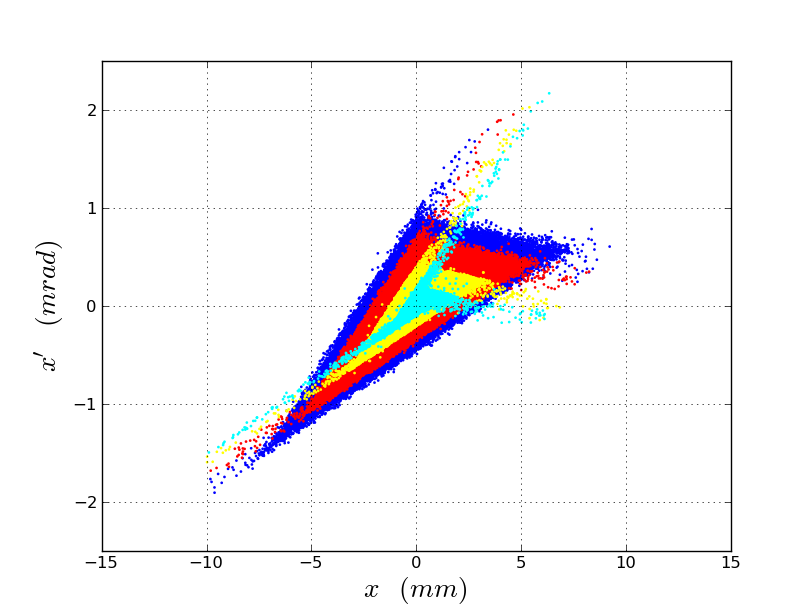
\includegraphics[width=.45\textwidth]{img/bump40.png}
    \label{fig:bump00}}
  \subfigure[After applying dynamic bumps]{
    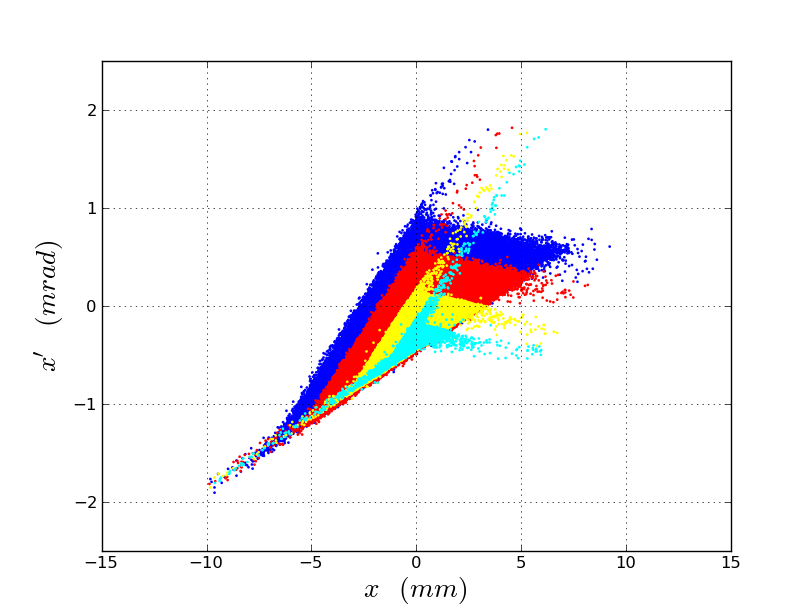
\includegraphics[width=.45\textwidth]{img/bump41.png}
    \label{fig:bump01}}
  \caption{\label{fig:bump0}Phase space plots of particles for 4 different extraction stages (100, 10000, 20000, 30000 turns): (a) before and (b) after applying dynamic bump corrections}
\end{figure*}

Fig.~\ref{fig:bump00} shows a phase space of particles for 4 different extraction stages.
As the separatrix is squeezed by increasing tune-quad strengths, unstable particles are streamed along branches of separatrices. 
The septum field region is formed on the [left] side of the vertical line (color: purple) at $x=10$ mm. 
The gray shadows on the plot are defined as the septum shadow regions in which particles will be considered as lost~\cite{m.pullia}.
Streams of unstable particles on the [leftmost] separatrix branch for each stage are entering the septum field region by crossing the septum foil line.
However, their entering angles are moving [upward] during the extraction processes.
An angle of the septum foil plane is aligned with an initial extraction stage.
Therefore, the alignment is only valid for few turns at the beginning, and there will be continuous misalignment of the septum foil plane later.
These result that more particles are entering the [upper] septum shadow region (color:gray shadow), and they will be lost.
Variations of angle coordinates at the septum entrance will eventually be seen at the experiment target with large horizontal angular spread of extracted beams.

In our case with a zero dispersion at the septum, there are two possible ways to have same entrance angle of the beam to the septum for different extraction stages.
One method is to compensate the beam angle by rotating the separatrix. This could be achievable by changing phases of two harmonic sextupole circuits.
The phase contributions of each harmonic circuit differs by about 90 deg, and these make phase adjustments doable.
However, particles' entrance angles for different extraction stages are same only if their $x$ coordinates are equal to the horizontal position of the septum foil at the entrance, $x_{ES}$.
In other words, their angles beyond $x_{ES}$ will be diverged.
These results in an asymmetric angular spread of extracted beams.

The other solution is to apply local orbit corrections using angle bumps throughout the spill.
With this method, extracted particles will have a symmetric angular spread during the spill as well as same entrance angles.
For resonant extraction from the Delivery ring, we choose a local orbit correction scheme.
Particles' orbit in the extraction beamline will be dynamically corrected with 4 bump magnets.
As a backup solution to prepare a failure of local bump corrections, the harmonics sextupole magnets and their power supplies are designed to preserve ramp capabilities.
In this paper, we will only discuss how local bump corrections are implemented, and detailed specifications for magnets and power supplies are presented in the Mu2e TDR~\cite{tdr}.

\begin{figure}[!tbp]
  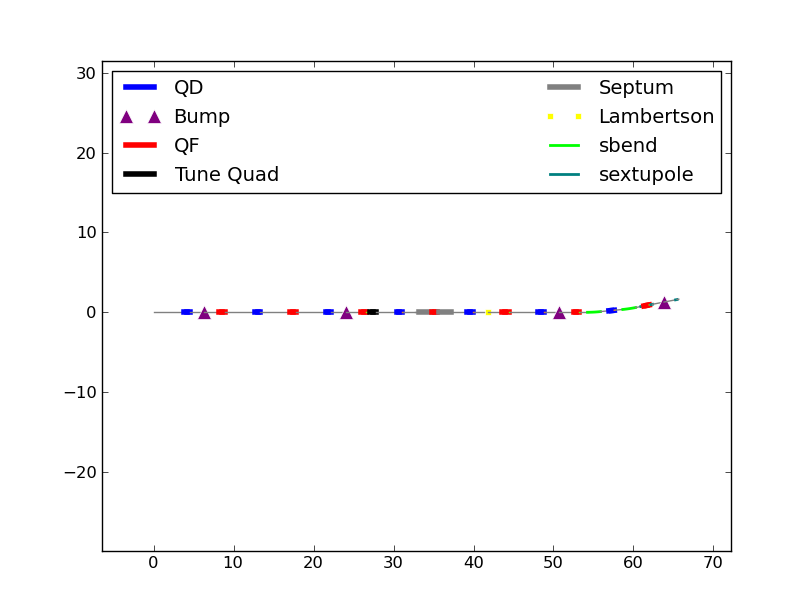
\includegraphics[width=.45\textwidth]{img/20140109-00.png}
  \caption{\label{fig:bump1}Schematic drawing of the external beamline with 4 local orbit bumps.}
\end{figure}

Using 4 dynamic bumps, we could align separatrices to reduce angular deviations at the entrance of the septum.
Fig.~\ref{fig:bump1} is a schematic drawing of 4 dynamic bump locations in the extraction beamline.
2 bumps are located at the upstream of septa, and the other 2 are at the downstream.
Upstream bumps kick particles so that the base of separatrices are aligned during the entire extraction period.
Then, downstream bumps will kick them back to original orbits.
Fig.~\ref{fig:bump01} presents a phase space plot of particles for different extraction stages after applying local orbit corrections.
All triangular distributions of particles are well aligned on their bases.
The [leftmost] branch arms are extended to the same direction, i.e., particles are entering the septum field region with the same angle.

Strengths of local orbit corrections can be easily obtained by applying the transfer matrix method with initial closed orbit conditions.
With the condition that the closed orbit is zero outside bumps, their strengths in time, $\theta_{i}(t)$ for $i=1,2,3,4$, are given by
\begin{equation}
  \begin{split}
  \theta_{1}(t) & = \sqrt{\frac{\beta_{s}}{\beta_{1}}}
               \frac{\sin(\psi_{s} - \psi_{2})}
                    {\sin(\psi_{2} - \psi_{1})}
               \left( - \Delta x_{s}^{\prime} (t) \right),
  \\ %\;\;\;
  \theta_{2}(t) & = \sqrt{\frac{\beta_{s}}{\beta_{2}}}
               \frac{\sin(\psi_{s} - \psi_{1})}
                    {\sin(\psi_{2} - \psi_{1})}
               \Delta x_{s}^{\prime} (t), \\
  \theta_{3}(t) & = \sqrt{\frac{\beta_{s}}{\beta_{3}}}
               \frac{\sin(\psi_{s} - \psi_{4})}
                    {\sin(\psi_{4} - \psi_{3})}
               \Delta x_{s}^{\prime} (t),
  \\ %\;\;\;\;\;\;\;\;\;\;
  \theta_{4}(t) & = \sqrt{\frac{\beta_{s}}{\beta_{4}}}
               \frac{\sin(\psi_{s} - \psi_{3})}
                    {\sin(\psi_{4} - \psi_{3})}
               \left( - \Delta x_{s}^{\prime} (t) \right),
  \end{split}
  \label{eqn:bump}
\end{equation}
where $\beta_{i}$'s are betatron functions at the septum($s$) and bumps($1,2,3,4$), $\psi_{i}$'s are betatron phase advances, and $\Delta x^{\prime}_{s} (t)$ is the required angle kicks of particles at the septum entrance as a function of time.
Fig.~\ref{fig:bump2} shows changes of bump strengths vs.~time.
Since particles' entrance angles to the septum are aligned to the initial extraction stage, bump strengths are zero at the beginning and are maximum at the end of extraction.
From Eqn.~\ref{eqn:bump}, we observed that strengths of bump magnets are getting smaller further when the distance of each pair for upstream and downstream bumps are closer.
Since each magnet is bounded between two quadrupoles, there are limitations in minimizing their strengths.

\begin{figure}[!tbp]
  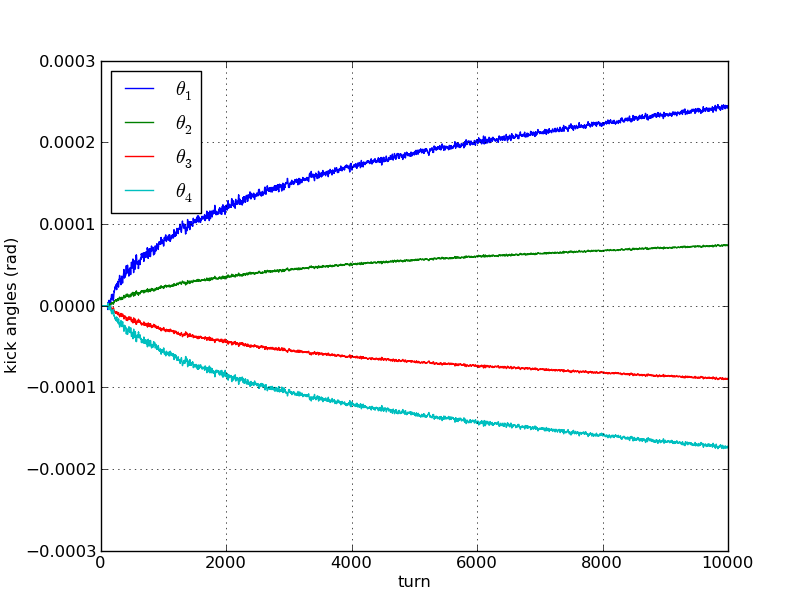
\includegraphics[width=.45\textwidth]{img/20140123-00.png}
  \caption{\label{fig:bump2}Strengths changes of dynamic bumps in time.}
\end{figure}

In Fig.~\ref{fig:bump3}, footprints of extracted particles at the entrance of the first septum are presented in phase space coordinates.
These are accumulations of extracted particles  with/without local orbit corrections throughout the entire extraction period.
Particles' coordinates are shifted to make them centered at the origin.
Particles (color:blue) survived from lost or scattered by septum components will be transferred to the 2nd septum, Lambertson magnet, and C-magnet.
They will be then extracted to the external beamline.
Particles (color:red) formed a thin line on the [right] hit the septum foil with 50$\mu$m at the entrance during the spill.
Some particles (color:purple) intersect the septum foil plane by entering the septum shadow region (color:gray shadow).
The last two kinds of particles are removed and considered as lost.
The horizontal phase space ellipses, which match the beam with 99.9\% containment, are plotted alongside.

Before applying local orbit corrections, the footprint has a wide angular spread and there are many beam losses due to crossing the foil plane as seen in Fig.~\ref{fig:bump30}.
However, Fig.~\ref{fig:bump31} shows a narrower angular thickness of the extracted particle distribution with dynamic orbit corrections.
The footprint of the extracted beam without the dynamic bumps is matched to an unnormalized emittance of [1.26]$\pi$mm-mrad and its matching horizontal betatron function is [9.1]m. The local orbit corrected beam has a [0.55]$\pi$mm-mrad emittance and [20.1]m betatron function.
After applying local orbit corrections, angular spreads of the beam also depend on the tune spread as the separatrix is squeezed.
The Delivery Ring has a nonzero chromaticity for the mixing of the coherent RFKO excitation~\cite{ipac11}.
Therefore, the chromatic tune spread causes a little spread of angle coordinates as seen in Fig.~\ref{fig:bump31}, while the overall emittance of the corrected beam is small compared to that of uncorrected beam.

\begin{figure*}[!tbp]
  \subfigure[Before applying dynamic bumps]{
    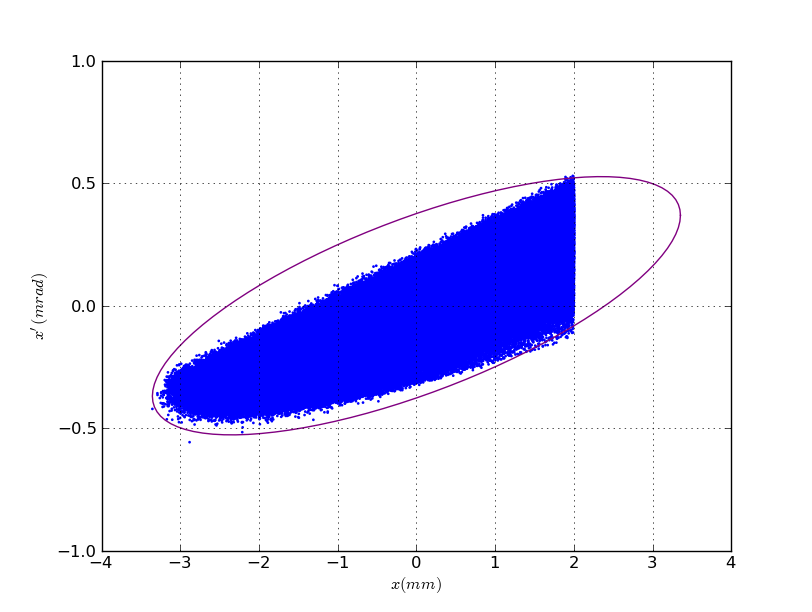
\includegraphics[width=.45\textwidth]{img/20140206-02.png}
    \label{fig:bump30}}
  \subfigure[After applying dynamic bumps]{
    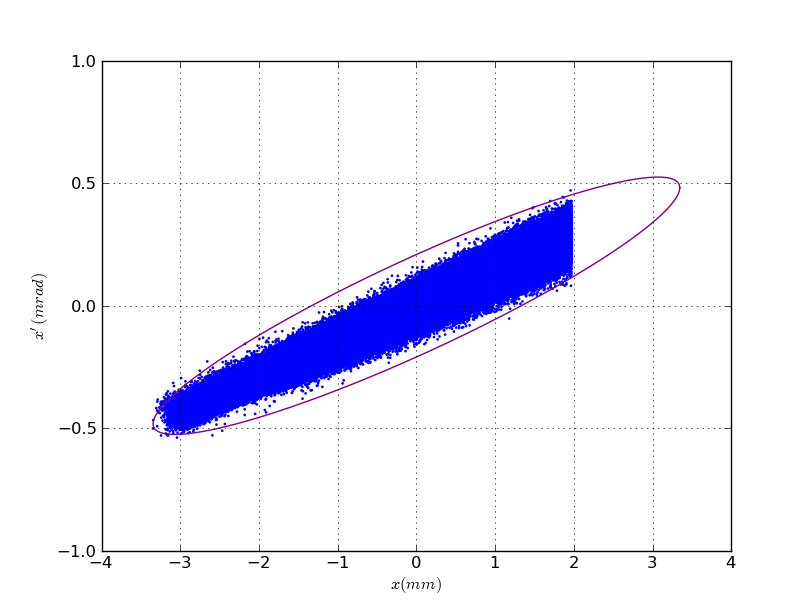
\includegraphics[width=.45\textwidth]{img/20140206-03.png}
    \label{fig:bump31}}
  \caption{\label{fig:bump3}Footprints of extracted particles with/without dynamic bumps.}
\end{figure*}

As described in the previous paper~\cite{mu2e}, Synergia2 has a septum aperture to detect particle losses by hitting a septum head or crossing a septum foil plane.
The rotation of the septum plane is taken into account in the model.
Fig.~\ref{fig:bump4} shows extraction simulation results of particle losses with/without local orbit corrections during the spill.
While ``hit\_septum1'' and ``hit\_septum2'' are losses by hitting the entrance of septum elements, ``cross\_septum1'' and ``cross\_septum2'' are losses by crossing septum foil planes for the 1st and 2nd septa, respectively.
``entire\_losses'' are a sum of turn-by-turn particle losses for each case.

Without dynamic angle corrections, septum planes are aligned only to the beginning of the extraction stage.
Therefore, beam losses are rising in time due to mismatching of the alignment (see Fig.~\ref{fig:bump40}).
When dynamic bumps correct the beam orbit, particles' entrance angles are well matched to septum foil planes.
In Fig~\ref{fig:bump41}, turn-by-turn particle losses are not changing much and are much smaller compared with no orbit corrections.
We also observed that losses at the 2nd septum with dynamic bumps are decreased.

\begin{figure*}[!tbp]
  \subfigure[Before applying dynamic bumps]{
    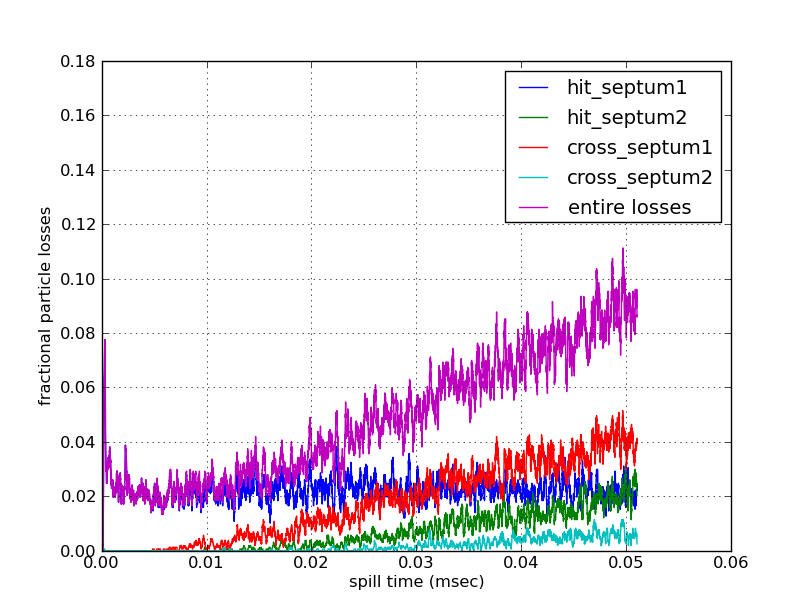
\includegraphics[width=.45\textwidth]{img/20140203-06.png}
    \label{fig:bump40}}
  \subfigure[After applying dynamic bumps]{
    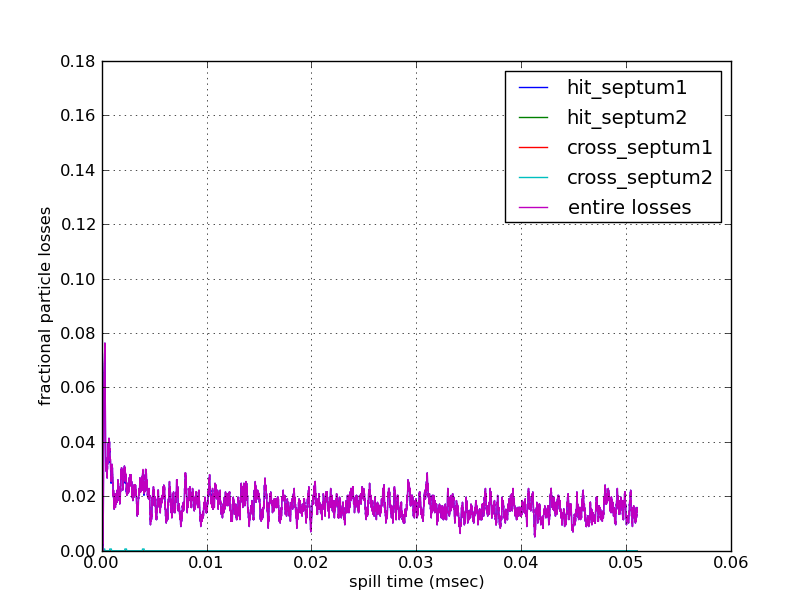
\includegraphics[width=.45\textwidth]{img/20140203-07.png}
    \label{fig:bump41}}
  \caption{\label{fig:bump4}Particle losses in time with/without dynamic bumps.}
\end{figure*}

\section{\label{sec:loss}Tracking of Particle Losses}


\clearpage

\section{\label{sec:arrival}Arrival Time Distribution}

\section{\label{sec:rfko}RFKO Beam Distribution Function}

\section{\label{sec:emit}Emittance Growth Rates with RFKO Beam Heating}

\section{\label{sec:conclusion}Conclusion}

\section{\label{thanks}Acknowledgments}

\begin{thebibliography}{77}

  \bibitem{tdr}
  Mu2e Technical Design Documentation

  \bibitem{mu2e}
  C.S. Park, ``Tracking Simulation of the Third-Integer Resonant Extraction for the Fermilab Mu2e Experiment,'' submitted to PRST-AB.

  \bibitem{ipac11}
  V. Nagaslaev, J.F. Amundson, J.A. Johnstone, C.S. Park, and S.J. Werkema, ``Third Integer Resonance Slow Extraction Using RFKO at High Space Charge,'' in IPAC 2011 proceeding.

  \bibitem{m.pullia}
  M. Pullia, thesis

\end{thebibliography}

\clearpage

\end{document}

%sagemathcloud={"zoom_width":100}